\chapter{Overview of radical inventions}\label{chap:inventions}

\section{Introduction} %TODO check count
In this chapter, we perform the assessment of five inventions based on the
framework described in \autoref{chap:intro}. \autoref{chap:imaging} already
described various breakthroughs in diagnostic medical imaging, but most of them
predate 1980. Fortunately researchers in the field have come up with plenty of
other innovations in the last thirty years, some of which will be detailed
below. We included one invention per imaging modality described, plus one more
related to computer aided diagnosis (CAD).

For each innovation, a technological definition is provided wherein the purpose
or goal is outlined, and the components plus their interactions are explained.
Next, the innovation is scored based on the assessment sheet in the appendix. Of
course the scores are substantiated with literature references where needed.

\section{Radiography invention: digital radiography}
A quick Google search on ``radiography breakthrough" suffices to show that
digital radiography is the most significant invention for basic radiography in
recent decades. As mentioned earlier in \autoref{ssec:recentradio}, digital
radiographs are much easier to store, copy, post-process and share compared to
their analogue siblings. Additionally, unlike radiographic film there is no potential
for over- or underexposure. Instead, the output can be rescaled as needed during
post-processing. Some techniques also allow for a reduced exposure of the
patient, minimizing the risk. The ubiquity of digital scanners these days prove
that the advantages outclass the disadvantages. However, these disadvantages do
exist. Analogue images have a very high inherent resolution, and by examining
them on a lightbox the contrast is unmatched by any kind of computer screen. In
addition, because analogue systems do not use digital electronics, there is no
electronic noise. Digital radiographs do not have necessarily to outclass their
analogue counterparts on these fronts, but they have to achieve a minimum level
to make sure their diagnostic value is not impaired.

\subsection{Defining the technology}
What makes radiography analogue or digital depends on kind of detector used.
Other parts of the scanner such as the X-ray source do not have to be altered
to make the transition. Furthermore, it is not one specific technology that
makes this transition possible. Various components are needed, and for each
of them there are some alternatives as well. On top of that, evolution in other
fields such as digital electronics and computer machinery had to be advanced
enough to take full advantage of the possibilities. 

\begin{figure}[ht]
\begin{center}
  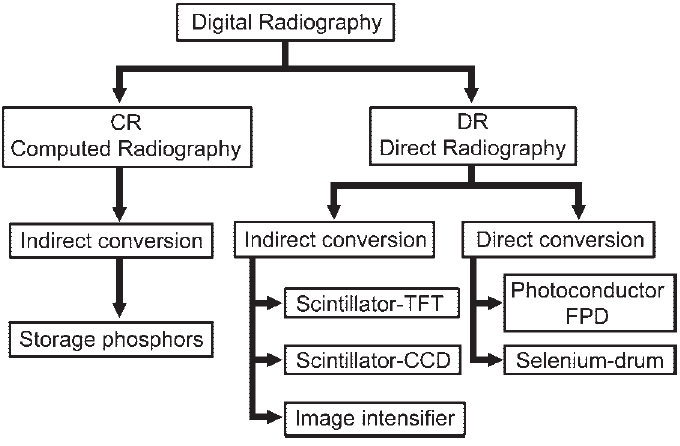
\includegraphics[width=\linewidth]{img/radiohierarchie.png}
  \caption{A systematic overview of various types of digital detectors. CCD =
  chargecoupled device, FPD = flat-panel detector, TFT = thin-film transistor.
  \cite{digitalradio}}
  \label{fig:radiohierarchie}
\end{center}
\end{figure} 

We first discuss the various types in greater detail using
\autoref{fig:radiohierarchie}. The first incarnation of digital radiography -
called computed radiography (CR) - used storage phosphor to temporarily store
the image information, and lasers to read out the values pixel by pixel at a later
stage \cite{digitalradio}. Unfortunately, the physical properties of storage
phosphors severely limited the resolution of the resulting image, reducing their
diagnostic value. The technology underwent many iterations, as shown in
\autoref{tbl:radiotime}.

\begin{table}[ht]
\begin{tabular}{l l}
\hline
Year & Development\\
\hline
1980 & Computed radiography (CR), storage phosphors\\
1987 & Amorphous selenium�based image plates\\
1990 & Charge-coupled device (CCD) slot-scan direct radiography (DR)\\
1994 & Selenium drum DR\\
1995 & Amorphous silicon�cesium iodide (scintillator) flat-panel detector\\
1995 & Selenium-based flat-panel detector\\
1997 & Gadolinium-based (scintillator) flat-panel detector\\
2001 & Gadolinium-based (scintillator) portable flat-panel detector\\
2001 & Dynamic flat-panel detector fluoroscopy�digital subtraction angiography\\
\hline
\end{tabular}
\caption{Timetable of developments in digital radiography \cite{digitalradio}.}
\label{tbl:radiotime}
\end{table}

The alternative to computed radiography is direct radiography (DR). It comes in
two forms, using either direct or indirect conversion. The direct form uses a
photoconductor to convert the incident photons to electrical charges. Typical
semiconductor materials used in photoconductors are amorphous Selenium (a-Se)
and Gadolinium (Gd). In earlier versions the photons were projected onto a
rotating drum and converted to electrical signals using an analog to digital
converter (ADC). Newer versions however use a flat panel detector (FDP) where
the ADC is swapped out for thin-film transistors (TFT, also used in LCD
displays). These TFTs are made of amorphous Silicon (a-Si). Because the used
materials have a very high intrinsic resolution, the final image resolution is
only limited by the quality of the underlying detector array.

\begin{figure}[ht]
\begin{center}
  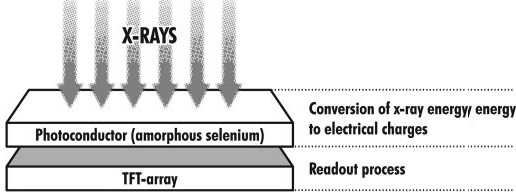
\includegraphics[width=\linewidth]{img/direct_FPD.png}
  \caption{Components of a direct conversion flat panel detector. \cite{digitalradio}}
  \label{fig:directfpd}
\end{center}
\end{figure}

In indirect conversion DR, an extra element is added between the X-rays and the
actual detector. A common example is a scintillator plate that converts X-rays
into visible light. Alternatively, an image intensifier (II) can be used to
amplify the light output. This light can than be captured more easily by a
charge-coupled device (CCD, also used in digital cameras) or a TFT. Because of
the extra step, the point spread function (PSF) increases and the resolution
suffers slightly.

A CCD chip is relatively small so it cannot under normal circumstances record a
whole image at once. Two alternatives are possible. One uses a lens to focus the
rays onto the smaller chip area, but this reduces the image quality. Another
uses a small collimated fan-shaped beam combined with a moving CCD detector.
This system performs comparable to FPDs. One drawback is that this elaborate
setup is not very mobile.

Instead of a CCD, TFTs can also be used in a similar fashion as in direct
conversion DR FPDs. Only this time a scintillator is added. These scintillators
use either Cesium Iodide (CsI) or Gd-based crystals. Contrary to Gd, CsI
crystals can be structured, improving the image quality. The trade-off is their
brittleness, making them less portable. The visible light they emit is then
captured by photo diodes and read out by a TFT array.

\begin{figure}[ht]
\begin{center}
  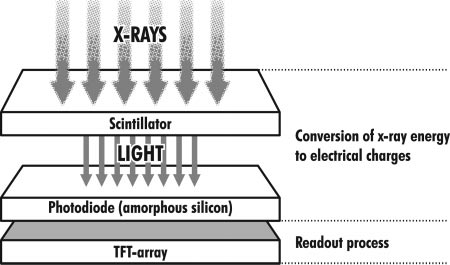
\includegraphics[width=\linewidth]{img/indirect_FPD.png}
  \caption{Components of an indirect conversion flat panel detector. \cite{digitalradio}}
  \label{fig:indirectfpd}
\end{center}
\end{figure}

For the actual assessment, we will focus on both direct and indirect FPDs.

\subsection{Assessing novelty in functionality}
Functionality-wise, we can distinguish between novelty in components and
combinations thereof on the one hand, and novelty in natural effects exploited
on the other hand.

\subsubsection{Novelty in components}
As explained above, digital radiography in general uses many of the same parts
as analogue radiography. Only the detector is fundamentally different. Of course
the real advantage of digitizing radiographs is what you can do with them
afterwards. However, that is out of the scope of this text, and we will
constrain ourselves to the hardware aspects for now.

The next question we ask ourselves is whether these new (combinations) of
components were already used before. The answer is yes. For example CCDs were
invented in 1969 at AT\&T Bell Labs (patents: US3792322,  US3796927) and first
used in digital cameras by 1975 \cite{solidstatesens}. On the other hand, the
combination of a scintillator with CCDs to capture X-rays was not used before. 

In the case of direct FPDs using TFTs, the results are similar. Engineers
experimented with them as early as 1971 for use in display equipment
\cite{lcdhistory}. To this day, they are almost exclusively used in LCD panels
and in digital radiography. In conclusion, they were used before, but mostly in
a field that is not closely related to medical imaging.

\subsubsection{Novelty in natural effects exploited}
Of course the primary natural effect exploited is that of the X-ray passing
through tissue. This has not changed with digital radiography. On the other
hand, the natural effects used in the digital detector are very distinct from
those in classic photographic film. Where such films fall under the
accomplishments of material science, modern digital recording equipment are made
possible by advances in the electronic and semiconductor industry. Obviously
these natural effects were exploited numerous times before by other digital
equipment, but not equipment related to medical imaging.

\subsubsection{Scores}
In \autoref{tbl:funcscores1} we give an overview of the scores on the various topics.

\begin{table}[h]
\centering
\begin{tabular}{l l}
\hline
\multicolumn{2}{|c|}{Novelty in functionality} \\
\hline
A. Novelty of components & B. Novelty in natural effects exploited\\
A1) 4 & B1) 8\\ 
A2) 5 & B2) 5\\ 
\hline
\end{tabular}
\caption{Novelty in functionality scores}
\label{tbl:funcscores1}
\end{table}

\subsection{Assessing novelty in knowledge origins}
Regarding knowledge origins (KOs), we can make a distinction between scientific
and technological origins. To find these KOs, we first provide a list of
problems that had to be solved for digital radiography to become feasible.

The main purpose is to somehow intercept the X-rays and translate their
intensities per pixel into a discrete values that can be processed by a
computer. To do so, they X-rays must first be converted to electrical charges,
which can then be interpreted as bits.

Problem 1: converting the X-ray intensities to bits

Problem 1.1: converting the X-rays to electrical charges

Solution 1.1a: direct conversion: use a photoconducting material (a-Se)

KO1: electromagnetism, semiconductors

Solution 1.1b: indirect conversion: use a scintillator (CsI) and photodiodes (a-Si)

KO2: electromagnetism, material science and semiconductors

Problem 1.2: converting the electrical charges to bits

Solution 1.2: use a TFT array

KO3: digital electronics (mostly transistors)

\subsubsection{Scores}
Electromagnetism falls under scientific origins. The use of electromagnetism
knowledge in medical imaging is certainly nothing special, so it receives low
scores.

The other origins fit better in the technological group. The use of digital
electronics and all related disciplines makes digital radiography what it is.
This warrants a high score, at least for the detector part. However, at
the time of invention the digital electronics industry was booming and
already widely in use in various other fields. In that regard it was only a
matter of time before someone came up with the idea to combine digital
electronics with radiography.

\autoref{tbl:origscores1} shows the scores.

\begin{table}[h]
\centering
\begin{tabular}{l l}
\hline
\multicolumn{2}{|c|}{Novelty in knowledge origins} \\
\hline
A. Novelty of scientific origins & B. Novelty of technological origins\\
A1) 2 & B1) 8\\ 
A2) 2 & B2) 5\\ 
\hline
\end{tabular}
\caption{Novelty in knowledge origins scores}
\label{tbl:origscores1}
\end{table}

\subsection{Assessing technological impact}
The last part of this digital radiography assessments looks into technological
impact. Impact can be split into three parts: performance increase,
technological accumulation and obsoleting previous technologies.

\subsubsection{Performance increase}
The goal of radiography is simply to make clear images that have a high
diagnostic value. To that end, spatial resolution, contrast and noise as
discussed in \autoref{sssec:imgquality} are all important. The aim of digital
resolution was not necessarily to do better in this regard, because analogue
images were already very detailed. If the quality is on par, we should consider
ourselves happy.

As explained above, resolution was a problem with computer radiography using
storage phosphors. However, the materials used in flat panel detectors all have
a high inherent spatial resolution. Only the size of the underlying TFT array
limits the final image resolution. Because analogue radiographs are not
expressed in number of pixels, the performance comparison is complicated.
However, tests performed by \cite{review} show that diagnostic value of analogue
and digital images are almost on par as long as the pixels are about 0.1mm in
size.

Contrast on the other hand is a serious problem for digital radiography. The
deep blacks of photographic film combined with the strong light from a lightbox
creates very high contrast. In comparison, radiologists now have to look at
images on their computer screen in a dark room. On the other hand, digital
radiography makes up for this defect by offering the possibility of
post-processing where it is not only possible to zoom in spatially, but also on
a certain intensity interval (using so-called grey-level transformations
\cite{suetens}). This way, contrast can be increased in one intensity interval
in exchange for lowering it in other intervals.

Noise-wise, the electronic circuits introduce additional electronic noise on top
of the electromagnetic noise. Fortunately, modern electronics can minimize the
former noise, as evident by our crisp digital photographs and big flat screens.

Other advances in performance include: lack of geometric distortion, no veiling
glare, uniform response across the field of view \cite{review}. In addition,
costs are reduces because expensive photographic film is no longer needed, and
time span is reduces because film development happens automatically and almost
instantly.

It is difficult to assign a single score to this component because of the many
issues at play. The image quality did not necessarily improve much, but this was
not the goal. The real performance increase is due to indirect opportunities
opened up by the digital image format. Therefore, in our opinion this still
deserves a fairly high score.

\subsubsection{Technological accumulation}
In this section we estimate the broadness, magnitude and novelty of the impact.

\paragraph{Broadness of impact}
The real breakthrough that made digital radiography possible was the
advent of digital electronics. This breakthrough had a very broad impact on
fields other than its own. Other fields looked directly at digital electronics,
rather than digital radiography, for possible innovations. That is why this
innovation does not score high on broadness of impact. It did however impact
related fields such as CT and PET.

\paragraph{Magnitude of impact}
Although the broadness of impact was not big, and it mostly concentrated on
highly related fields, the magnitude was considerable. In fact, computed
tomography would not even be possible if it were not for the invention of
digital detectors. The same goes (to a lesser extent) for detectors used in
nuclear medicine imaging.

\paragraph{Novelty of impact}
The novelty of impact of digital radiography is very low because other
technologies that never used digital electronics before, got their ideas from
digital electronics in general, not specifically from digital radiography.

\subsubsection{Obsoleting previous technologies}
The last aspect of impact assessment regards obsoleting previous technologies,
i.e.\ analogue radiography. According to \cite{review} and \cite{suetens}, this
has indeed happened. Few radiology departments still stick with analogue systems
because of their lower cost and extreme reliability, but most of the world has
permanently moved on. Not only in radiography, but also in related disciplines
such as CT and PET.

\subsubsection{Scores}
\autoref{tbl:impactscores1} shows the scores.

\begin{table}[h]
\centering
\begin{tabular}{l l l}
\hline
\multicolumn{3}{|c|}{Technological impact} \\
\hline
A. Performance increase & B. Tech. accumulation & Obsoleting previous tech.\\
A) 8 & B1 a) 3 --- b) 1 & C) 10\\ 
     & B2 a) 8 --- b) 7 & \\
     & B3 a) 1 --- b) 1 & \\
\hline
\end{tabular}
\caption{Technological impact scores}
\label{tbl:impactscores1}
\end{table}

\section{CT invention: Electron-beam CT} %US 4352021 A (Boyd, 1982)
Our next assessment deals with an innovation related to computed tomography. In
particular, we take a closer look at Electron-beam Computed Tomography (EBCT),
also know as Ultrafast CT.

\subsection{Defining the technology}
Traditional CT scanners have an X-ray tube embedded in the toroid body. By
mechanically rotating the tube along with the detector, projections from an
arbitrary angle can be captured.

EBCT also needs to be able to capture projections from any angle, but takes
another route. Remember that in a regular X-ray tube current flowing through the
cathode releases electrons. The electrons are accelerated towards the anode by
applying a voltage across the tube. When the electrons hit the anode at high
speed, they release part of their energy as X-rays. The same principle is used
in EBCT, except that the tube is physically split up in two dedicated parts. One
is the cathode or electron gun and is placed along the patient's longitudinal
axis. The other is the anode and is shaped in a semi-ring around the patient.
Using magnetic fields, the electrons fired from the cathode are deflected onto this
ring, where they produce X-rays that can be captured by a detector array as
usual \cite{suetens}. \autoref{fig:ebctscanner} illustrates this.

\begin{figure}[ht]
\begin{center}
  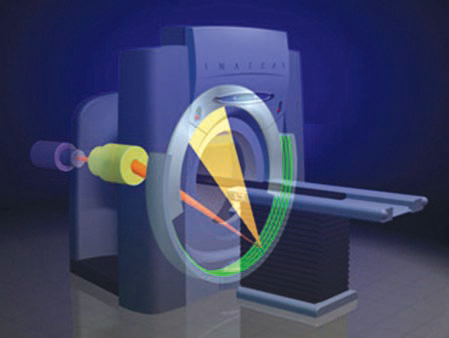
\includegraphics[width=\linewidth]{img/EBCT.png}
  \caption{Rendering of an EBCT scanner's inner workings \cite{suetens}.}
  \label{fig:ebctscanner}
\end{center}
\end{figure}

The main advantage of this setup is that the X-ray source rotation is no longer
mechanical. This allows for faster sweeps, which in turn make it easier to image
moving structures such as the heart. In traditional CT scanners, this movement
would cause blurring in the final image, and thus a loss of diagnostic value.
One very prominent EBCT application is the detection of calcifications from
atherosclerosis in the coronal arteries (i.e., coronary artery disease)
\cite{ultrafastcad}. These are very close to the heart, and can move by about
five times their own diameter every heartbeat.

More recently, these EBCT scanners have received strong competition from
multislice helical CT scanners. The latter enjoy a widespread adoption and are
also less costly (partly due to economies of scale and increased competition).
However, their rotation speed still cannot match that of Ultrafast CT
\cite{ultravshelical}. In addition, this techniques requires a lower dose
compared to traditional CT, and much lower than a CT angiography
\cite{ultralowdose}. The latter is a common alternative for diagnosing coronary
artery disease when an EBCT scanner is not available.

In conclusion, this technique is promising for non-invasive detection of
coronary heart disease, but it has too many unsolved problems to replace general
purpose CT scanners \cite{multictbook}.

\subsection{Assessing novelty in functionality}

\subsubsection{Novelty in components}
As outlined above, the components are largely the same as in conventional CT
scanners. Only their location is different. One additional component is the coil
to generate the deflecting magnetic field. Such electromagnets were used before
in imaging, particularly in MRI, but for a very different purpose.

\subsubsection{Novelty in natural effects exploited}
The same story applies for novelty in natural effects exploited: few new effects
except bending of the electron beam using magnetic fields. The same principle
was used much earlier in Cathode Ray Tube (CRT) monitors and televisions.

\subsubsection{Scores}
In \autoref{tbl:funcscores2} we give an overview of the scores on the various
topics.

\begin{table}[h]
\centering
\begin{tabular}{l l}
\hline
\multicolumn{2}{|c|}{Novelty in functionality} \\
\hline
A. Novelty of components & B. Novelty in natural effects exploited\\
A1) 3 & B1) 3\\ 
A2) 5 & B2) 5\\ 
\hline
\end{tabular}
\caption{Novelty in functionality scores}
\label{tbl:funcscores2}
\end{table}

\subsection{Assessing novelty in knowledge origins}
Again, we look into the problems that had to be solved to find the knowledge
origins. We only look at the problems that are different in comparison to a
traditional CT scanner.

Problem 1: deflect the electron beam onto the anode ring.

Solution 1: use magnetic fields (electric field deflection only works for small angles)

KO1: electromagnetism, CRT monitors

Problem 1.1: overcoming Coulomb repulsion to obtain proper beam focus

Solution 1.1: leak nitrogen into vacuum chamber \cite{ebctelectric}

KO2: charged particle optics

Problem 2: synchronise imaging with heart rhythm

Solution 2: use ECG equipment

KO3: biomedical sensors, signal processing

\subsubsection{Scores}
Electromagnetism, charged particle optics and signal processing can be
considered scientific origins, while the others are technological in nature.

Note that using ECG equipment to synchronise imaging with the heart rhythm is
not new. It was occasionally used before in various other imaging modalities
\cite{suetens}.

\autoref{tbl:origscores2} shows the scores.

\begin{table}[h]
\centering
\begin{tabular}{l l}
\hline
\multicolumn{2}{|c|}{Novelty in knowledge origins} \\
\hline
A. Novelty of scientific origins & B. Novelty of technological origins\\
A1) 4 & B1) 5\\ 
A2) 1 & B2) 1\\ 
\hline
\end{tabular}
\caption{Novelty in knowledge origins scores}
\label{tbl:origscores2}
\end{table}

\subsection{Assessing technological impact}
\subsubsection{Performance increase}
As outlined above, EBCT is very useful for mainly one thing: imaging the heart
and its periphery. However, there are serious drawbacks that do not make it
useful as a general purpose CT scanner. For example, due to the new geometry
X-ray scatter cannot be reduced as effectively. This in turn generates extra
artifacts on the resulting image. The electron gun also has limited power making
it inadequate for higher dosage (i.e., higher contrast) studies \cite{multictbook}.

\subsubsection{Technological accumulation}
Surprisingly, we were unable to identify any newer invention based on EBCT.
Various other applications using electron beams were checked, such as electron
microscopes and electron beam lithography, but none seem to be based on
innovations in EBCT. This may be caused by the relative obscurity of EBCT
outside of medical imaging fields.

\subsubsection{Obsoleting previous technologies}
EBCT has definitely not obsoleted previous technologies. Its application area is
simply too narrow for many hospitals to warrant such an expensive purchase.
Instead, older and cheaper but less effective methods are still used more often
to diagnose coronary artery disease. Examples include a CT angiography, exercise
stress tests but also invasive (catheter) examinations.

\subsubsection{Scores}
\autoref{tbl:impactscores2} shows the scores.
\begin{table}[h]
\centering
\begin{tabular}{l l l}
\hline
\multicolumn{3}{|c|}{Technological impact} \\
\hline
A. Performance increase & B. Tech. accumulation & Obsoleting previous tech.\\
A) 5 & B) N/A & C) 2\\ 
\hline
\end{tabular}
\caption{Technological impact scores}
\label{tbl:impactscores2}
\end{table}

\section{MRI invention}
Normally we only consider inventions from 1980 onwards, but for this section we
would like to make an exception. The invention of the MRI scanner itself was a
veritable breakthrough, and still happened relatively close to 1980. Because we
already had a close look at MRI in \autoref{sec:mri}, we will skip the
technology definition and go straight to the assessment.

\subsection{Assessing novelty in functionality}
\subsubsection{Novelty in components}
The purpose of MRI scanners is largely the same as that of CT scanners: create
cross-sectional images to look into patient's bodies without using invasive
techniques. The essential components of CT are the X-ray source and the
detector. With MRI, we again have a signal source and a signal detector.
However, this time the source is a large electromagnet, and the detector is a
quadrature detector.

Electromagnets are used in various other technologies to do the same thing:
generate magnetic fields. Examples include motors, generators, transformers,
relays and loudspeakers. In that sense the choice was not very special.

Similarly, quadrature detectors are used universally whenever signal
demodulation is required \cite{quadrature}. Remember that MRI operates in the
radio frequency range, so ordinary radio technology could be repurposed for use
in these scanners.

In summary, these components were not used in medical imaging before the advent
of MRI. Yet, once it was decided to exploit radio waves and magnetic fields, the
choice of components was rather trivial.

\subsubsection{Novelty in natural effects exploited}
MRI has one thing in common with the other imaging modalities discussed: they
all use electromagnetic radiation in one form or another. Nevertheless, the way
this natural effect is exploited here is considerably different from other
modalities. In radiography and CT, we measure the X-ray attenuation when
traveling through the human body. With nuclear medicine, we essentially detect
photons emitted by radioactive materials. MRI on the other hand influences and
measures the magnetic properties of tissues, in particular the proton density,
the $T_1$ time or the $T_2$ time.

In a way, every researcher that ever worked on imaging based on magnetic fields
contributed to the eventual creating of MRI. Of course some groups took a
slightly different turn (e.g. measuring properties of electrons instead of
protons), but their larger goal was the same. To our knowledge no one
experimented with these specific magnetic properties for any other purposes.

\subsubsection{Scores}
In \autoref{tbl:funcscores3} we give an overview of the scores on the various
topics.

\begin{table}[h]
\centering
\begin{tabular}{l l}
\hline
\multicolumn{2}{|c|}{Novelty in functionality} \\
\hline
A. Novelty of components & B. Novelty in natural effects exploited\\
A1) 10 & B1) 8\\ 
A2) 3 & B2) 8\\ 
\hline
\end{tabular}
\caption{Novelty in functionality scores}
\label{tbl:funcscores3}
\end{table}

\subsection{Assessing novelty in knowledge origins}
Once again, we start with a list of problems and corresponding solutions.

Problem 1: measure proton density in tissue

Problem 1.1: align net magnetization vectors

Solution 1.1: generate a large magnetic field

KO1: electromagnetism

Problem 1.1.1: increase field strength, lower power consumption

Solution 1.1.1: superconductivity by extreme cooling

KO2: physics (cryogenics), material science

Problem 1.2: measure magnetization vector

Solution 1.2a: disturb equilibrium with the appropriate pulse sequence

KO3: theory from electromagnetism, but to our knowledge never exploited before

Solution 1.2b: record relaxation phenomena using quadrature detector

KO4: analogue electronics, radio equipment 

Problem 2: localize position using signal

Solution 2: apply a magnetic field gradient

KO5: electromagnetism, gradients recently used in \cite{nanogradients1,
nanogradients2}, older: \cite{oldgradients}.

\subsubsection{Scores}
None of these knowledge origins, except the usage of specific pulses, is out of
the ordinary. Radio equipment is also a new technological origin, but its
purpose in other inventions is very similar. That is why in
\autoref{tbl:origscores3} we give low scores except for this technological
origin.

\begin{table}[h]
\centering
\begin{tabular}{l l}
\hline
\multicolumn{2}{|c|}{Novelty in knowledge origins} \\
\hline
A. Novelty of scientific origins & B. Novelty of technological origins\\
A1) 2 & B1) 6\\ 
A2) 2 & B2) 7\\ 
\hline
\end{tabular}
\caption{Novelty in knowledge origins scores}
\label{tbl:origscores3}
\end{table}

\subsection{Assessing technological impact}
\subsubsection{Performance increase}
Although we have portrayed MRI as the successor to CT in the section above, this
is not completely true. MRI allows us to visualize things we could not before
with CT. For example, cancerous tissue is sometimes easier to spot on MRI scans.
Whereas on CT scans the attenuation properties of both tissue types might be
very similar, malignant tumors appear to exhibit a larger $T_1$ value than
surrounding tissue \cite{mrihistory}.

On the other hand, CT has the advantage when it comes to visualizing bone.
Because it contains few free hydrogen atoms, it is very difficult to spot on an
MRI scan. X-rays however are ideal for this type of diagnosis.

In conclusion, it is very difficult to unilaterally award the performance
trophy to either side. 

\subsubsection{Technological accumulation}
\paragraph{Broadness of impact}
MRI generated a lot of spin-off technologies, including Magnetic Resonance
Angiography (MRA), Magnetic Resonance Spectroscopy (MRS) and functional MRI
(fMRI). These are of course all part of the same imaging family, and we could
not find any impact outside of this family in the literature. Perhaps
mining through patents can show some interesting results. 

\paragraph{Magnitude of impact}
Although the broadness is limited, the magnitude of impact is substantial.
Especially for the direct spin-offs listed above, but also indirectly through
the spin-offs of those spin-offs.

\paragraph{Novelty of impact}
As stated above, we only identified direct impact on its immediate spin-off
technologies. The degree of novelty is thus very low.

\subsubsection{Obsoleting previous technologies}
As stated before in \autoref{ssec:mrifuture}, MRI has not replaced CT, but is
expected to gain more traction in the future. For now, the two technologies are
complimentary: each is better for a specific subcategory of diagnostic imaging. 

\subsubsection{Scores}
\autoref{tbl:impactscores3} shows the final scores.

\begin{table}[h]
\centering
\begin{tabular}{l l l}
\hline
\multicolumn{3}{|c|}{Technological impact} \\
\hline
A. Performance increase & B. Tech. accumulation & Obsoleting previous tech.\\
A) 5 & B1 a) 4 --- b) 2 & C) 3\\ 
     & B2 a) 8 --- b) 8 & \\
     & B3 a) 1 --- b) 1 & \\
\hline
\end{tabular}
\caption{Technological impact scores}
\label{tbl:impactscores3}
\end{table}

\section{Nuclear medicine invention: 18F-FDG tracers}
In this assessment related to nuclear medicine we focus on something slightly
unusual. Not a component or new technique used in the scanner, but on one of the
popular tracers used during such examinations: $^{18}$F-FDG tracers.

\subsection{Defining the technology}
PET scanners work by detecting positrons formed by the decay of radioactive
tracers, as explained in \autoref{chap:nuclearimg}. The most commonly used
isotope is fluorine-18. It is very suited for PET because it almost exclusively
emits positrons when decaying to oxygen-18. Its half life of 110 minutes gives
it another attractive property.

%The first incarnation of these kind of glucose-based tracers was 

However, the fluorine isotope is only responsible for the emission of positrons,
it cannot be absorbed by or transported in the human body on its own. That is
where 2-deoxy-2-fluoro-D-glucose or, more conveniently fluorodeoxyglucose (FDG),
comes into play. One of its hydroxyl (-OH) groups can be replaced by
fluorine-18. Because it is analogous to normal glucose, its uptake in the body
is also similar. However, unlike normal glucose it cannot be completely
metabolised as long as the fluorine isotope is present. Instead, it gets stuck
in the cells until the fluorine decays into oxygen and it can form a hydroxyl
group again.

When the tracer is injected into the body, a PET scanner can visualize its
distribution throughout the various tissues. This way, physicians can monitor
glucose metabolism and spot abnormalities or deviations. Those can be caused by
tumors for example, which typically grow very fast and consequently need lots of
energy. Brain activity can also be measured regionally because active parts of
the brain tend to metabolise more glucose.

Synthesis of FDG is possible in a number of ways, but most are rather
sophisticated. 

%impact: neuroscience, oncology

%1948: NO, Fick principle, cerebral bloodflow (global)
%1977: Sokoloff, C14-glucose [20]
%1979: Reivich [21], FDG, Ido et al. [22]
%uses: table 1

\subsection{Assessing novelty in functionality}

\subsubsection{Novelty in components}
The F-FDG tracer is a composite made out of both FDG and fluorine-18. Earlier
tracers also used FDG, but the isotopes were different. Carbon-14 was a popular
choice \cite{radiopharma}. The fluorine-18 seems to be exclusively used as a
radioactive tracer. It is sometimes also combined with other molecules, for
example to track dopamine instead of glucose \cite{fluorodopa, fdopamine}.
Another isotope (fluorine-19) is used as a contrast agent in MRI studies.

The first paper describing the synthesis of F-FDG already mentioned specific
usage as a radiopharmaceutical \cite{firstF-FDG}. To our knowledge, it has not
been used outside this context. Within this context however, it was used towards
many different goals in biomedical research such as neuroscience and oncology. 

\subsubsection{Novelty in natural effects exploited}
The tracer isotope exploits radioactive decay, more specifically positron
emission decay. Considering PET works exclusively with positron emission decay,
this is no special feat. However, what makes fluorine-18 special is that it
hardly has any other decay mechanisms and that its half life has the ideal
length for PET studies.

The second natural effect exploited is how the human body treats FDG very
similar to normal glucose.

\subsubsection{Scores}
In \autoref{tbl:funcscores4} we give an overview of the scores on the various
topics.

\begin{table}[h]
\centering
\begin{tabular}{l l}
\hline
\multicolumn{2}{|c|}{Novelty in functionality} \\
\hline
A. Novelty of components & B. Novelty in natural effects exploited\\
A1) 6 & B1) 3\\ 
A2) 2 & B2) 1\\ 
\hline
\end{tabular}
\caption{Novelty in functionality scores}
\label{tbl:funcscores4}
\end{table}

\subsection{Assessing novelty in knowledge origins}
To make F-FDG work, a number of problems had to be overcome.

Problem 1: find a tracer that emits positrons

Solution 1: the following isotopes are known to emit positrons:  carbon-11,
nitrogen-13, oxygen-15, fluorine-18, sodium-22, aluminium-26, potassium-40, 
and iodine-121

KO1: nuclear physics

Problem 1.1: find an isotope that easily combines with lots of molecules 

Solution 1.1: carbon-11 and fluorine-18 \cite{radiopharma}

KO2: biochemistry

Problem 1.2 find an isotope that has a suitable half life for PET studies

Solution 1.2 fluorine-18

KO3: nuclear physics

Problem 2: find a suitable transport molecule that mimics glucose

Solution 2: replace one hydroxyl group in normal glucose with an isotope 

KO4: biochemistry, pharmacology

\subsubsection{Scores}
\autoref{tbl:origscores4} shows the scores. Note that there are no technical
knowledge origins. This is a consequence from the rather unique category of
innovation radiopharmaceuticals belong to. The scientific knowledge origins on
the other hand are rather straightforward for these kinds of applications.

\begin{table}[h]
\centering
\begin{tabular}{l l}
\hline
\multicolumn{2}{|c|}{Novelty in knowledge origins} \\
\hline
A. Novelty of scientific origins & B. Novelty of technological origins\\
A1) 1 & B1) N/A\\ 
A2) 1 & B2) N/A\\ 
\hline
\end{tabular}
\caption{Novelty in knowledge origins scores}
\label{tbl:origscores4}
\end{table}

\subsection{Assessing technological impact}
\subsubsection{Performance increase}
Performance of positron emission tracers is difficult to quantify. Remember that
in nuclear medicine the image quality is of secondary importance. More important
is the fidelity of the tracer. It should properly visualize the biochemical and
physiological processes, glucose metabolism in our case. Empirical tests
confirmed that FDG is effectively processed in the same manner as normal glucose
in the body, and that PET scans highlight regions where glucose metabolism is
expected to be higher (brains, kidneys, tumors) \cite{radiopharma}. Earlier
incarnations such as $^{11}$C-glucose also achieved this. Unfortunately, because
of the short half life of just 20 minutes, images had to be taken before the
tracer had the chance to diffuse properly.

\subsubsection{Technological accumulation}
\paragraph{Broadness of impact}
The success of F-FDG inspired the production of several other tracers. One
example is a tracer called F-fluoro-DOPA for studying dopamine utilization
\cite{radiopharma}.

However, the biggest impact by far was on research in the fields of medicine and
physiology. This tracer opened up lots of new possibilities, and application in
oncology, neuroscience, virology etc. \cite{fdgresearch1, fdgresearch2}.

\paragraph{Magnitude of impact}
As stated before, the invention of FDG led to many spin-off tracers, and each of
those tracers has multiple spin-offs itself. The magnitude of impact is thus
significant.

\paragraph{Novelty of impact}
Fields such as virology could traditionally not make use of imaging modalities,
because viruses are simply too small to be seen. However, FDG-related
technologies in combination with PET scanners have allowed researchers to
finally see what exactly goes on at this microscopic level \cite{fdgresearch2}.

On the other hand, most of the impact was on fields that already made extensive
use of imaging modalities, such as oncology or neuroscience.

\subsubsection{Obsoleting previous technologies}
These days PET and F-FDG are so intricately linked that it is hard to imagine a
time before this tracer was used. Yet, research in this field is still ongoing
and very active. Other biochemical processes obviously require different
transport molecules, and not all of them are compatible with fluorine-18. That
is why many other tracers are still in use today. But when it comes to
visualizing glucose metabolism, F-FDG seems to be the gold standard for now
\cite{radiopharma}.

\subsubsection{Scores}
\autoref{tbl:impactscores4} shows the scores.

\begin{table}[h]
\centering
\begin{tabular}{l l l}
\hline
\multicolumn{3}{|c|}{Technological impact} \\
\hline
A. Performance increase & B. Tech. accumulation & Obsoleting previous tech.\\
A) 7 & B1 a) 7 --- b) 3 & C) 8\\ 
     & B2 a) 7 --- b) 6 & \\
     & B3 a) 4 --- b) 3 & \\
\hline
\end{tabular}
\caption{Technological impact scores}
\label{tbl:impactscores4}
\end{table}

\section{CAD invention: machine learning techniques for mammography}
For this last assessment, we draw from the field of Computer-aided Detection and
Diagnosis. For the rest of this section, we will focus on the usage of machine
learning techniques for CADe in mammography. Breast cancer is one of the
deadliest cancers among women today, but fortunately early detection
significantly improves the chances of survival \cite{mammoairecent}. To detect
breast cancer, phycisians look for calcifications, masses and architectural
distortions on high resolution radiographs (mammograms). Traditionally, every
image is checked by at least two radiologists to increase sensitivity. This is
known as the second reader principle. However, this approach effectively doubles
the workload of the radiology department. Perhaps more than in any other
medical field, CAD can help radiologists by acting as a surrogate second reader
for mammograms. \cite{mlinmedical}.

One particular application where CAD has proven its worth, is in the detection
of microcalcifications in mammograms. These are small calcium deposits of 0.05mm
to 1mm in size that appear as bright white spots on the scan. They are known to
appear in 30-50\% of all breast cancer cases, and are thus an important
indicator. Due to their variable shape, brightness and size, they can be
difficult to detect in the surrounding tissue \cite{mlinmedical}.

Note that - unlike tangible inventions - software algorithms are not so
straightforward to assess using the radical innovation framework. For example,
algorithms typically do not exploit natural effects directly (but computers do).
However, we will make an effort to make a meaningful assessment regardless.

%\cite{mammoai}

\subsection{Defining the technology}
As explained in \autoref{ssec:cadadv}, machine learning comprises a large group
of methods and techniques. We are specifically interested in (binary)
classifiers to determine whether a particular structure on a mammogram is
suspicious enough. The exact nature of this classifier - whether it is a Support
Vector Machine (SVM) or Random Forests (RF) or anything else - is of little
interest for this assessment. We will simply look at them as one group with one
goal.

When assessing this technology, we will compare it to earlier incarnations of
CAD software without machine learning elements, and - where appropriate - with
manual diagnosis by a physician.

\subsection{Assessing novelty in functionality}
Because we are dealing with software algorithms, we can only assess the novel
functionality based on novelty in components, not on novelty in natural effects
exploited. 

\subsubsection{Novelty in components}
In \autoref{ssec:cadtech}, we discussed the generic scheme that most CAD systems
follow. Each of these steps can be considered a separate component in the
algorithm. In our case, step III and IV are replaced by machine learning
algorithms.

Of course these algorithms were used before in a variety of other applications,
but not necessarily related to diagnostic medical imaging
\cite{machinelearningapps}. 

\subsubsection{Scores}
In \autoref{tbl:funcscores5} we give an overview of the scores on the various
topics.

\begin{table}[h]
\centering
\begin{tabular}{l l}
\hline
\multicolumn{2}{|c|}{Novelty in functionality} \\
\hline
A. Novelty of components & B. Novelty in natural effects exploited\\
A1) 5 & B1) N/A\\ 
A2) 4 & B2) N/A\\ 
\hline
\end{tabular}
\caption{Novelty in functionality scores}
\label{tbl:funcscores5}
\end{table}

\subsection{Assessing novelty in knowledge origins}
As usual, we start by listing problems encountered during development of this
invention, and present the proposed solution and its related knowledge origin.
We again follow the five step detection scheme introduced before. 

Problem 1: detect abnormalities in mammograms

Problem 1.1: segment the region of interest

Solution 1.1: trivial, the mammogram only contains the region of interest

Problem 1.2: enhance abnormalities

Solution 1.2: use traditional image processing and computer vision methods
(e.g.\ convolution filters)

KO1: image processing

Problem 1.3: detect and segment abnormalities

Problem 1.3.1: detect abnormalities

Solution 1.3.1: use an appropriately trained machine learning classifier

KO2: statistics, artificial intelligence, machine learning

Problem 1.3.2: segment abnormalities

Solution 1.3.2: use traditional image processing and computer vision methods
(e.g.\ region growing)

KO3: image processing

Problem 1.4: perform feature analysis and classification

Solution 1.4: use an appropriately trained machine learning classifier

KO4: statistics, artificial intelligence, machine learning

Problem 1.5: reduce false positives

Solution 1.5: use traditional false positive reduction methods

KO5: statistics, machine learning

\subsubsection{Scores}
Of the listed knowledge origins, we classify statistics as scientific, and
the rest as technological.

Statistics forms the fundamental basis for almost all machine learning
algorithms. Some more primitive image processing techniques also explicitly use
statistical theory, but most do not. The radiologists that perform a manual
diagnosis use their advanced human visual system instead of relying on
statistics.

Of the technological knowledge origins, machine learning is by definition the
only new element compared to earlier methods.

\begin{table}[h]
\centering
\begin{tabular}{l l}
\hline
\multicolumn{2}{|c|}{Novelty in knowledge origins} \\
\hline
A. Novelty of scientific origins & B. Novelty of technological origins\\
A1) 6 & B1) 3\\ 
A2) 1 & B2) 5\\ 
\hline
\end{tabular}
\caption{Novelty in knowledge origins scores}
\label{tbl:origscores5}
\end{table}

\subsection{Assessing technological impact}
\subsubsection{Performance increase}
Already in 1990, \cite{cadsynergy} proved using observer studies that
radiologists' performance in detecting microcalcifications could increase when
using CAD systems, even if the number of false positives at the time were still
fairly high. The review article \cite{cadhistory} looked into various large
scale studies regarding CAD in mammography, and found that all of them reported
an increase in detection performance compared to pre-CAD diagnosis. Remember
that performance is this context is the combined performance of physician plus
computer, not computer alone. It should be mentioned that other studies found no
performance gain, or even a performance decrease \cite{mammocadbad}, but they
seem to be in the minority. They particularly lament the high number of false
positives, claiming that these cause more unnecessary examinations and
consequently an increase in medical insurance expenditures.

\subsubsection{Technological accumulation}
false positive reduction
\paragraph{Broadness of impact}
Machine learning is generally application-agnostic and thus a very versatile
technique used in a variety of fields, from the financial world over social
networks to medical applications. In fact, CAD was fairly late to jump on the
machine learning bandwagon \cite{mlinmedical}. Nonetheless, a lot of related
research is performed by biomedical scientists. This research is often generic
enough in nature to potentially be applied to other fields again. Unfortunately,
researchers outside of the medical field tend to ignore medical journals in
favor of their own field-specific alternatives. This severely degrades the
possible cross-pollination across fields, and in turn the broadness of impact.
This is evident by the lack of medical literature citations from outside the
field.

\paragraph{Magnitude of impact}
Globally speaking, the medical field only accounts for a relatively small slice
of all machine learning research. Consequently, most breakthroughs will
originate elsewhere, negatively impacting the magnitude of direct and
indirect impact of CAD on unrelated applications.

\paragraph{Novelty of impact}
Due to the versatility of machine learning, there is a lot of potential
for novelty of impact. But again, because of invisible walls surrounding the
medical field, we could not locate specific applications that drew from
biomedical machine learning research.

\subsubsection{Obsoleting previous technologies}
Within three years of FDA approval, about 10\% of of U.S. facilities switched to
CAD technology\footnote{\url{http://www.nih.gov/news/pr/apr2007/nci-04b.htm}}.
CAD technology using machine learning has not yet obsoleted conventional
mammography diagnosis, although performance definitely increases when employed.
Some physicians are simply reluctant to rely on technology for performing their
diagnosis. This will require a change in mindset, which is a long-term endeavor.
On top of that, these systems imply an additional cost on top of the already
expensive imaging equipment. Perhaps integrating them as modules in PACS as
suggested by \cite{cadhistory} will speed up their adoption. Because of these
reasons, researchers believe it is only a matter of time before such methods are
used globally.

\subsubsection{Scores}
\autoref{tbl:impactscores5} shows the scores.

\begin{table}[h]
\centering
\begin{tabular}{l l l}
\hline
\multicolumn{3}{|c|}{Technological impact} \\
\hline
A. Performance increase & B. Tech. accumulation & Obsoleting previous tech.\\
A) 7 & B1 a) 3 --- b) 5 & C) 4\\ 
     & B2 a) 3 --- b) 2 & \\
     & B3 a) 3 --- b) 2 & \\
\hline
\end{tabular}
\caption{Technological impact scores}
\label{tbl:impactscores5}
\end{table}

\section{Conclusion} %TODO most/least radical
In this chapter, we presented the results of the assessment of various
innovations related to diagnostic medical imaging. The most radical innovation
clearly was \ldots and the least radical \ldots.

We have tried to make this assessment as detailed as possible. However, medical
imaging is a very complex matter, and even our introduction in
\autoref{chap:imaging} - much like many a review paper - just barely scratch the
surface of all underlying methods and technologies. These details only become
apparent when hands-on work is performed by scientists and researchers in the
field. Consequently, these details will only be present in the most detailed
literature and of course in patent applications. We fear that this discrepancy
in level of detail will significantly hamper comparison with the automated
patent analysis.

The way the framework is built also seems to favor automatic patent based
analysis over manual assessment. The questions on the assessment sheet map
nicely to data that can be extracted from patents. On the other hand, manually
finding an answer to these questions without looking at patent data has proven
to be challenging.

In addition, the 1980 limit made it significantly more difficult to go back to
the real breakthrough invention, the so-called seed. For example, FDG in nuclear
medicine was certainly a breakthrough but it would have been more interesting to
go back further and see who first managed to bring nuclear physics together with
biochemistry and truly invent radiopharmacology.

%medical imaging: inventions seem to ``stay in the family''

%CAD: research used in other (3D) image processing applications

%difficult to go back to the source/seed with 1980 limit